
\section{Principal Component Analysis on Faces}
% Now we will perform PCA on images of faces and see how reducing the latent dimensions of our images affects the images reconstructions. First, start by uncommenting the code below to retrieve the faces dataset.
\subsection{Part 1: PCA with SVD and Resulting Eigenfaces}
\begin{enumerate}
    \item To check the outputs of your PCA functions, report the singular values here.
\begin{table}[H]
	\centering
	\begin{tabular}{@{}|c|c|c|c|c|c|@{}}
		\toprule
		\multicolumn{6}{|c|}{\textbf{Singular Values for PCA on Face dataset}} \\ \midrule
		86.701965  & 66.46528  & 50.15517  & 39.722527 & 33.757385 & 31.568754 \\ \midrule
		27.678606  & 25.354534 & 24.862415 & 22.975147 & 22.44062  & 21.298525 \\ \midrule
		19.838667  & 19.02967  & 18.317488 & 17.568378 & 17.033203 & 16.045595 \\ \midrule
		15.42673   & 15.356074 & 14.85018  & 13.929341 & 13.577002 & 13.410842 \\ \midrule
		13.130961  & 12.957497 & 12.735859 & 12.511106 & 12.019814 & 11.801411 \\ \midrule
		11.265183  & 11.012788 & 10.689299 & 10.276611 & 10.056747 & 9.988401  \\ \midrule
		9.814747   & 9.709447  & 9.4375105 & 9.3004675 & 9.055668  & 8.954327  \\ \midrule
		8.786291   & 8.701313  & 8.537433  & 8.454362  & 8.376851  & 8.342043  \\ \midrule
		8.121107   & 8.044209  &           &           &           &           \\ \bottomrule
	\end{tabular}
\end{table}
    \item Please describe what the eigenfaces look like. What do you expect to observe with the eigenfaces associated with lower eigenvalues?
    \newline
    \newline
    The eigenfaces represent abstractions of human features which explain the most variance within the dataset of images. The variance explained by each eigenface successively decreases for each eigenface, by definition of PCA.
    \item Please insert your eigenfaces output here.
\begin{figure}[H]
\centering
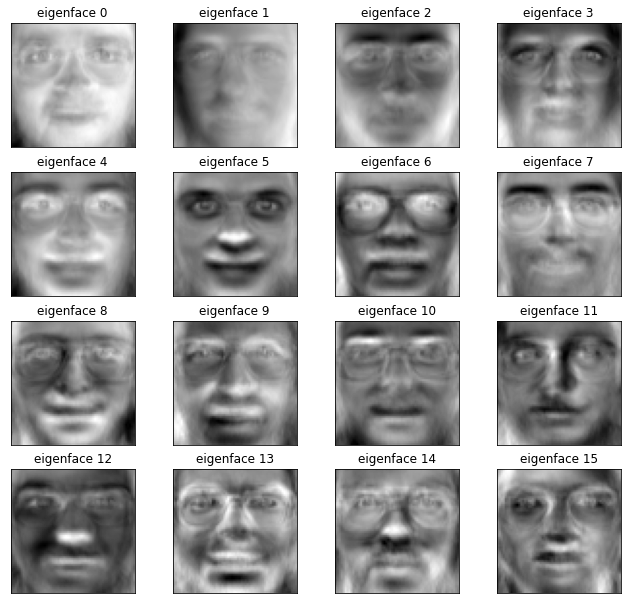
\includegraphics[width=.6\textwidth]{templates/eigenfaces}
\caption{Eigenfaces.}
\label{fig:my_label}
\end{figure}
\end{enumerate}
\subsection{Part 2: Reconstructing Faces}
\begin{enumerate}
    \item Paste in the reconstructed faces plot. Compare the reconstructed images to the original images. How are they similar and how are they different? Shortly explain why they are different?
    \begin{figure}[H]
    	\centering
    	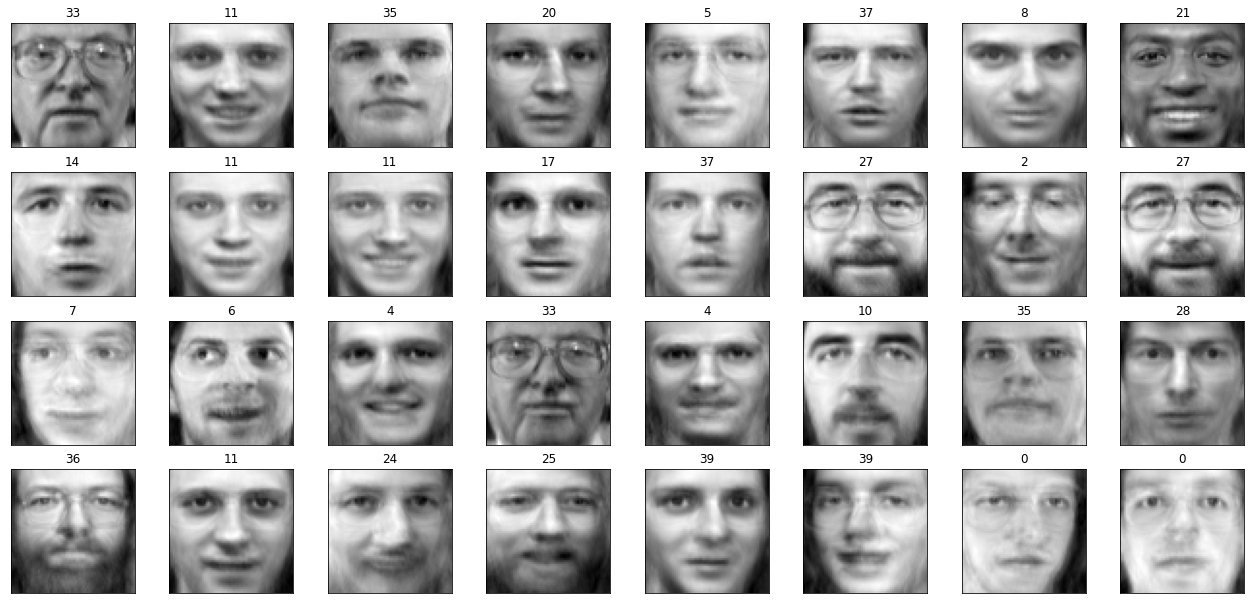
\includegraphics[width=1\textwidth]{templates/reconstructed_faces}
    	\caption{Reconstructed faces.}
    	\label{fig:my_label}
    \end{figure}
Similarities: The reconstructed images retain defining characteristics and structure of the human face.
Differences:
\begin{enumerate}
\item The reconstructed faces have lost variance in some features such as width and roundness of face, definition of nose, etc.
\item Lost nuances in facial expressions and pose such as jaw position.
\item New features such as definition of glasses got added on to faces even when the original image did not feature glasses.
\end{enumerate}
    \item What do you expect to see from the reconstructed images as the number of principal components chosen for PCA increases / decreases? Please explain why.
\newline
\newline
As the number of principal components increases, the reconstructed faces start to resemble the original faces to a greater degree, since the Principal component space starts to resemble the original data space to a closer degree.

Since PCA is a lower dimensional representation of the original data space, some clarity of the images will still be lost, but the number of principal components controls how close the reconstructed images will be to the original images.    
\end{enumerate}
\subsection{Part 3: Variance Explanation}
\begin{enumerate}
    \item How do you expect (based on theory; please be precise!) the plot of variance explained as the number of components to relate to the eigenvalues of the corresponding components?
    \newline\newline
The plot of cumulative variance explained is directly related to the eigenvalues of the corresponding components added to the model.

This is mathematically explained by the fact that the eigenvalue of a principal component is a measure of the variance described by that component.
    \item What is the relation between reconstruction error and the variance explained?
    \newline\newline
    Reconstruction error is inversely correlated to explained variance since as the explained variance increases, the principal component space captures more variance of the original dataset, reducing the reconstruction error.
    \item Insert the three line plots of explanation vs. number of
    components, descending eigenvalues vs. number of components, and reconstruction error vs. number of components here.
    
\begin{figure}[H]
\centering
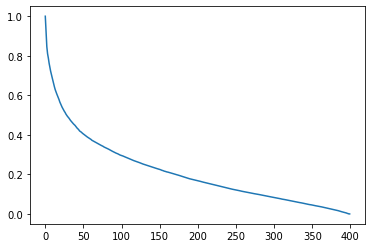
\includegraphics[width=0.5\textwidth]{templates/var_plot1}
\caption{Explanation vs. number of components.}
\label{fig:my_label}
\end{figure}

\begin{figure}[H]
	\centering
	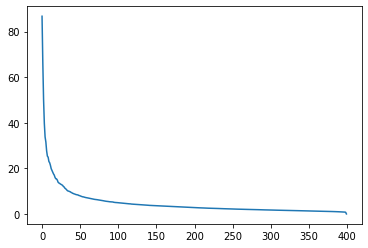
\includegraphics[width=0.5\textwidth]{templates/var_plot2}
	\caption{Descending eigenvalues vs. number of components.}
	\label{fig:my_label}
\end{figure}

\begin{figure}[H]
	\centering
	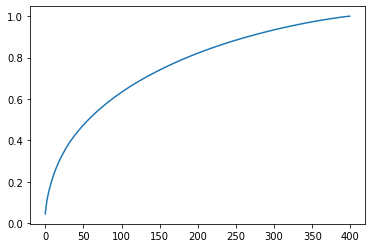
\includegraphics[width=0.5\textwidth]{templates/var_plot3}
	\caption{Reconstruction error vs. number of components.}
	\label{fig:my_label}
\end{figure}

\end{enumerate}